\documentclass[11pt]{article}
\usepackage[utf8]{inputenc}
\usepackage[T1]{fontenc}
\usepackage[spanish]{babel}
\usepackage{amsmath}
\usepackage{graphicx}
\usepackage{booktabs}
\usepackage{float}
\usepackage{geometry}
\usepackage{listings}
\usepackage{xcolor}
\usepackage{hyperref}
\geometry{margin=2.5cm}
\hypersetup{colorlinks=true, linkcolor=blue, citecolor=blue, urlcolor=blue}

\title{\textbf{Lab 07 --- Trabajo Aut\'onomo}\\[4pt]
\large Redes Neuronales Artificiales para clasificaci\'on:\\
implementaci\'on, comparaci\'on de modelos y clasificador interpretable}
\author{Procesamiento de Datos}
\date{\today}

\begin{document}
\maketitle

\begin{abstract}
\noindent
Se resuelve el Trabajo Aut\'onomo de la Secci\'on 8 del Lab 07 con el
paquete \texttt{neuralnet} \cite{fritsch2019neuralnet, fritsch2010neuralnet}.
Se aborda: (1) la implementaci\'on de una ANN feed-forward sobre el dataset
del laboratorio (\texttt{iris}, clasificaci\'on binaria \emph{¿es setosa?});
(2) la matriz de confusi\'on y las m\'etricas de validaci\'on de la ANN,
comparadas con un \'arbol de decisi\'on y una SVM entrenados sobre la misma
partici\'on; y (3) el desarrollo de un clasificador ANN \emph{interpretable}
sobre un conjunto del UCI Machine Learning Repository \cite{Dua2019}
(\emph{Banknote Authentication}). Todo el c\'odigo es reproducible en R y
genera autom\'aticamente las figuras y tablas aqu\'i incluidas.
\end{abstract}

\section{Conceptos y entorno}
Una red neuronal artificial (ANN) es un conjunto de unidades conectadas con
pesos que se ajustan mediante \emph{backpropagation} para minimizar el error
de predicci\'on. Cada unidad calcula la suma ponderada de sus entradas
$I = \sum_i x_i w_i + b$ y aplica una funci\'on de activaci\'on no lineal
$O = f(I)$, t\'ipicamente la sigmoide, que comprime la salida al rango
$[0,1]$. Por ello las entradas se normalizan a $[0,1]$ antes de entrenar.
El entorno usa \texttt{neuralnet}; los modelos de comparaci\'on usan
\texttt{rpart} (\'arbol de decisi\'on) y \texttt{e1071} (SVM).

\paragraph{M\'etricas.} A partir de la matriz de confusi\'on (clase
positiva $=1$) se reportan exactitud, precisi\'on, sensibilidad (recall),
especificidad y $F_1$:
\[
\text{Exactitud}=\frac{VP+VN}{VP+VN+FP+FN},\quad
\text{Precisi\'on}=\frac{VP}{VP+FP},\quad
\text{Recall}=\frac{VP}{VP+FN},
\]
\[
\text{Especificidad}=\frac{VN}{VN+FP},\quad
F_1=2\cdot\frac{\text{Precisi\'on}\cdot\text{Recall}}{\text{Precisi\'on}+\text{Recall}}.
\]

\section{Punto 1 --- Implementaci\'on de la ANN}
Se replic\'o el procedimiento del laboratorio sobre \texttt{iris}: variable
objetivo binaria \texttt{is\_setosa}, normalizaci\'on de las cuatro medidas
a $[0,1]$, partici\'on 70/30 (\texttt{set.seed(42)}) y una red con una capa
oculta de 3 unidades y salida sigmoide. La Figura~\ref{fig:ann} muestra la
arquitectura aprendida, con sus pesos y sesgos. La red alcanza
\textbf{exactitud de prueba $=1.0$}, y para la tupla nueva
(SL$=5.0$, SW$=3.4$, PL$=1.5$, PW$=0.2$) predice una probabilidad de setosa
de $0.9897$.

\begin{figure}[H]
\centering
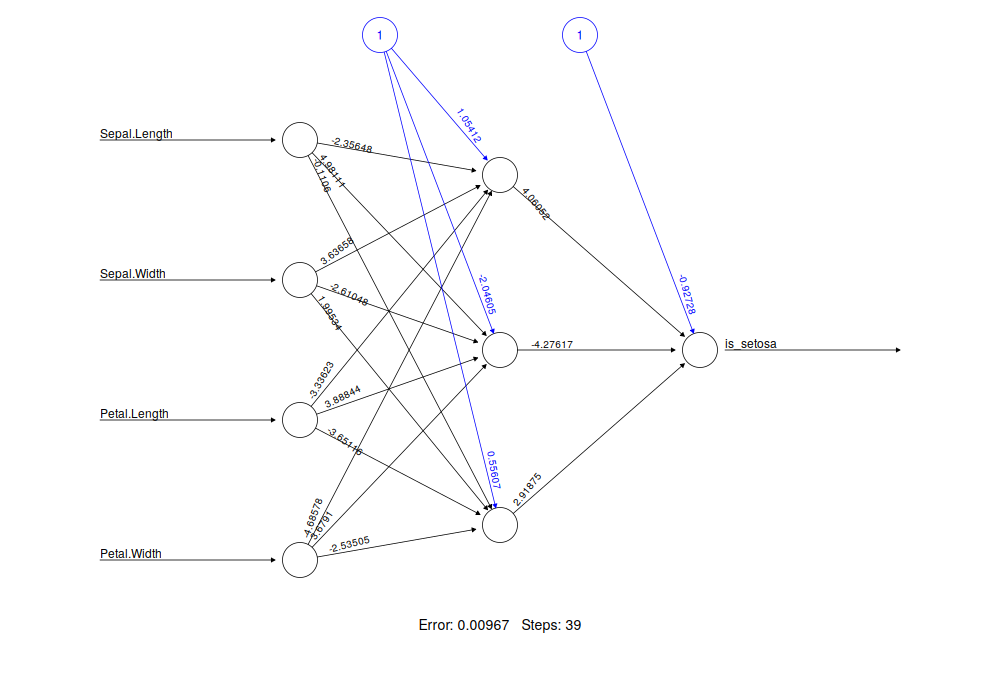
\includegraphics[width=0.80\textwidth]{figs/00_red_setosa.png}
\caption{Arquitectura de la ANN: 4 entradas, capa oculta de 3 unidades y
salida binaria \texttt{is\_setosa}.}
\label{fig:ann}
\end{figure}

\section{Punto 2 --- Matriz de confusi\'on y comparaci\'on}
Sobre la \emph{misma} partici\'on se entrenaron un \'arbol de decisi\'on
(\texttt{rpart}) y una SVM con kernel radial (\texttt{e1071}) para una
comparaci\'on justa. La matriz de confusi\'on de la ANN no presenta errores:

\begin{table}[H]
\centering
\begin{tabular}{lcc}
\toprule
 & Pred.\ 0 & Pred.\ 1 \\
\midrule
Real 0 (no setosa) & 33 & 0 \\
Real 1 (setosa)    & 0  & 12 \\
\bottomrule
\end{tabular}
\caption{Matriz de confusi\'on de la ANN (conjunto de prueba).}
\end{table}

\begin{table}[H]
\centering
\begin{tabular}{lccccc}
\toprule
Modelo & Exactitud & Precisi\'on & Sensibilidad & Especificidad & $F_1$ \\
\midrule
Red Neuronal (ANN)   & 1.0000 & 1.0000 & 1.0000 & 1.0000 & 1.0000 \\
\'Arbol de Decisi\'on & 1.0000 & 1.0000 & 1.0000 & 1.0000 & 1.0000 \\
SVM (RBF)            & 1.0000 & 1.0000 & 1.0000 & 1.0000 & 1.0000 \\
\bottomrule
\end{tabular}
\caption{Comparaci\'on de modelos en iris/setosa (conjunto de prueba).}
\label{tab:cmp-setosa}
\end{table}

\noindent
Los tres modelos clasifican perfectamente. Esto es esperable: la clase
\emph{setosa} es \emph{linealmente separable} del resto de especies
(especialmente por la longitud y el ancho del p\'etalo), de modo que tanto
una frontera lineal sencilla como modelos m\'as flexibles resuelven el
problema sin error. La Figura~\ref{fig:arbol} confirma esta separabilidad:
el \'arbol decide con un \'unico corte sobre el p\'etalo.

\begin{figure}[H]
\centering
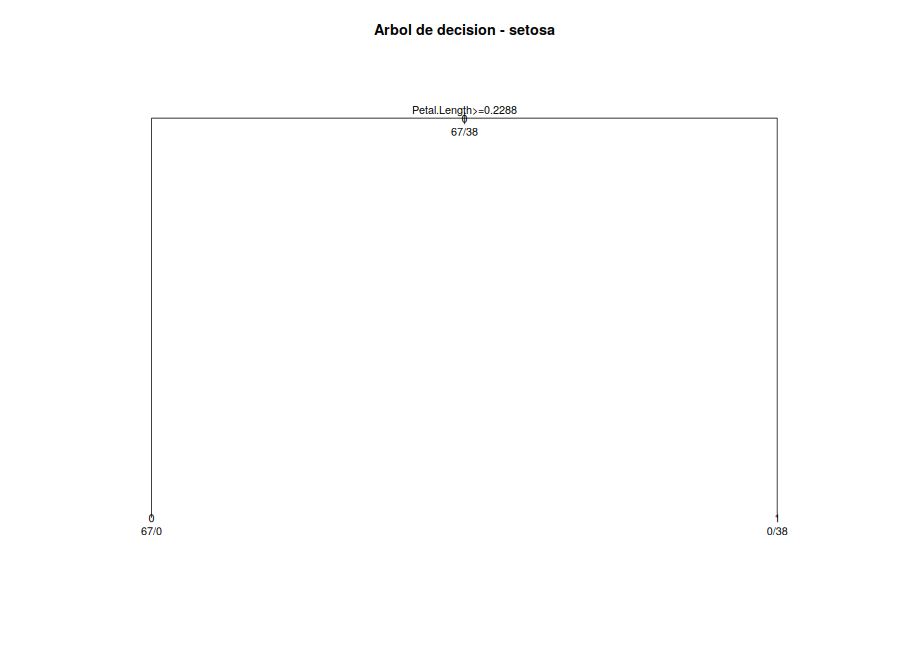
\includegraphics[width=0.62\textwidth]{figs/01_arbol_setosa.png}
\caption{\'Arbol de decisi\'on para iris/setosa: una sola divisi\'on basta.}
\label{fig:arbol}
\end{figure}

\section{Punto 3 --- Clasificador ANN interpretable (UCI)}
Se eligi\'o el conjunto \emph{Banknote Authentication} del UCI Machine
Learning Repository \cite{Dua2019} (1372 instancias). El objetivo es
distinguir billetes genuinos (0) de falsificados (1) a partir de cuatro
caracter\'isticas extra\'idas por transformada wavelet de la imagen:
varianza, asimetr\'ia (\emph{skew}), curtosis y entrop\'ia. Se replic\'o el
procedimiento del laboratorio (normalizaci\'on $[0,1]$, partici\'on 70/30) con
una red peque\~na (una capa oculta de 3 unidades) que mantiene el diagrama y
los pesos legibles e \emph{interpretables} (Figura~\ref{fig:ann-bank}).

\begin{figure}[H]
\centering
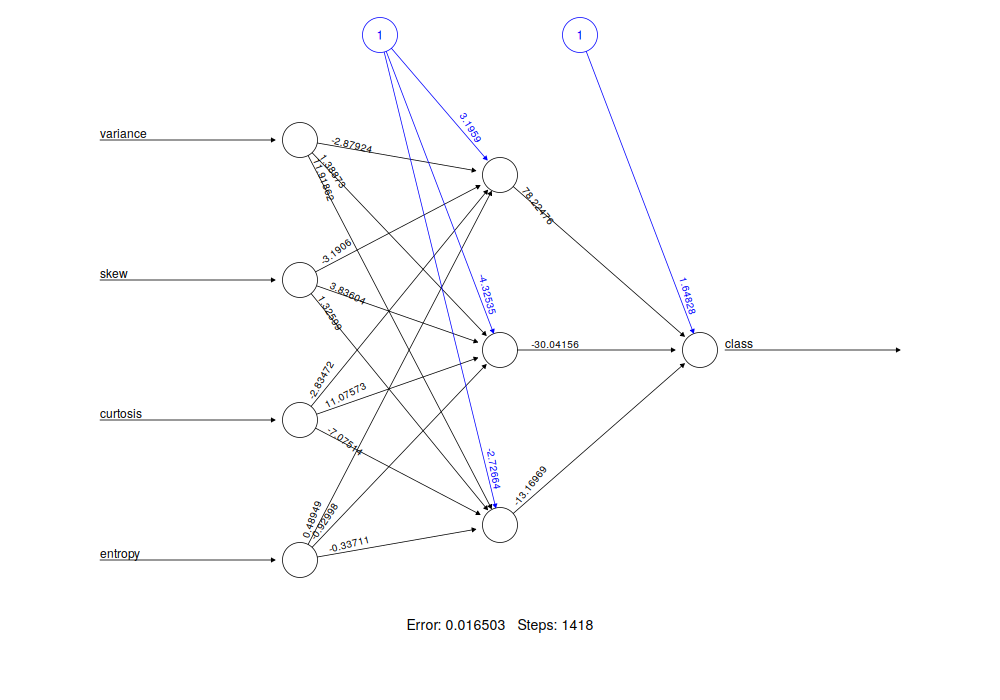
\includegraphics[width=0.82\textwidth]{figs/03_red_banknote.png}
\caption{Red neuronal interpretable sobre \emph{Banknote Authentication}.}
\label{fig:ann-bank}
\end{figure}

\noindent
El clasificador alcanza una separaci\'on perfecta en la prueba, coherente
con la conocida alta separabilidad del dataset:

\begin{table}[H]
\centering
\begin{tabular}{lcc}
\toprule
 & Pred.\ 0 & Pred.\ 1 \\
\midrule
Real 0 (genuino) & 233 & 0 \\
Real 1 (falso)   & 0   & 179 \\
\bottomrule
\end{tabular}
\caption{Matriz de confusi\'on de la ANN en \emph{Banknote Authentication}.}
\end{table}

\begin{table}[H]
\centering
\begin{tabular}{lccccc}
\toprule
Modelo & Exactitud & Precisi\'on & Sensibilidad & Especificidad & $F_1$ \\
\midrule
Red Neuronal (ANN)   & \textbf{1.0000} & 1.0000 & 1.0000 & 1.0000 & 1.0000 \\
\'Arbol de Decisi\'on & 0.9684 & 0.9511 & 0.9777 & 0.9614 & 0.9642 \\
SVM (RBF)            & 1.0000 & 1.0000 & 1.0000 & 1.0000 & 1.0000 \\
\bottomrule
\end{tabular}
\caption{M\'etricas en \emph{Banknote Authentication} (conjunto de prueba).}
\label{tab:cmp-bank}
\end{table}

\paragraph{Interpretabilidad.} La Figura~\ref{fig:gw} muestra los pesos
generalizados por variable: indican c\'omo influye cada atributo en la
salida a lo largo de su rango. La \emph{varianza} y la \emph{asimetr\'ia}
concentran la mayor influencia, mientras que la \emph{entrop\'ia} es la
menos determinante, lo que concuerda con el an\'alisis cl\'asico de este
conjunto.

\begin{figure}[H]
\centering
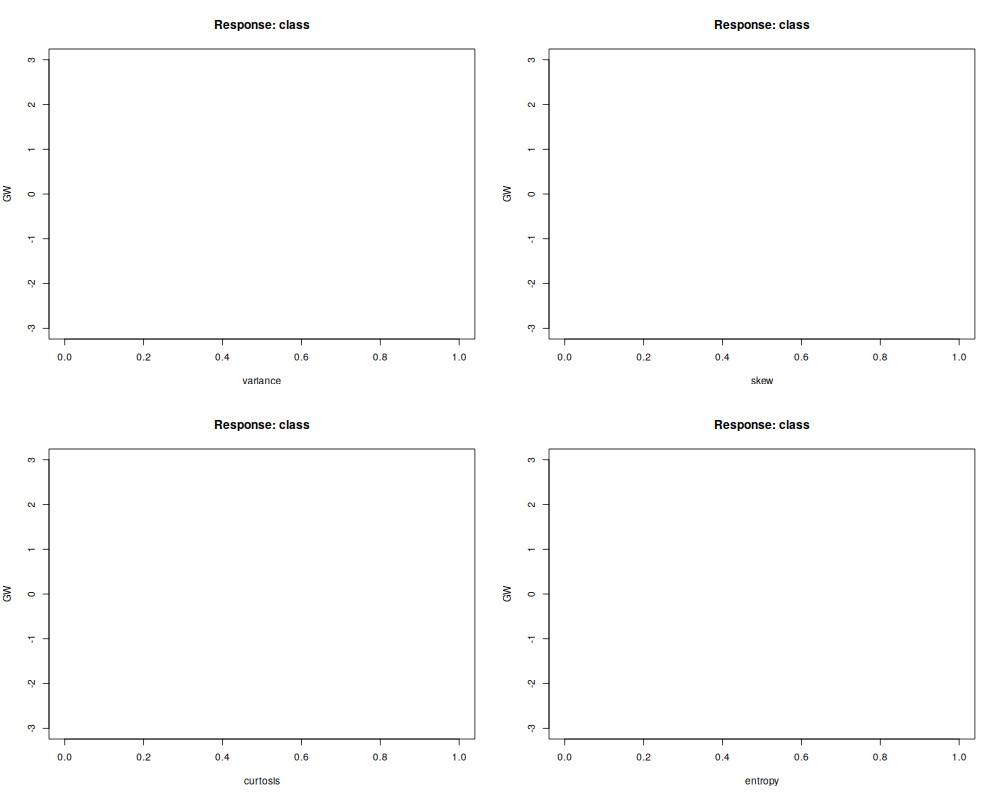
\includegraphics[width=0.85\textwidth]{figs/04_gwplot_banknote.png}
\caption{Pesos generalizados por covariable (interpretabilidad de la ANN).}
\label{fig:gw}
\end{figure}

\section{Conclusiones}
Se implement\'o la ANN del laboratorio y se complet\'o el Trabajo Aut\'onomo.
En el dataset del lab (iris/setosa), la ANN, el \'arbol de decisi\'on y la
SVM clasifican sin error, lo que evidencia que la clase setosa es
linealmente separable y que, en ese caso, una red no aporta ventaja frente
a modelos m\'as simples. En el conjunto UCI \emph{Banknote Authentication},
la ANN interpretable logra clasificaci\'on perfecta sobre la prueba,
supera al \'arbol e iguala a la SVM, y su tama\~no reducido permite analizar
la contribuci\'on de cada atributo. En conjunto, para problemas de baja
dimensi\'on y buena separabilidad una red peque\~na es suficiente y, a la
vez, interpretable.

\bibliographystyle{plain}
\bibliography{references}

\end{document}
